\documentclass[10pt]{article}

\usepackage{amsmath}
%
\usepackage{amssymb}
%
\usepackage{enumerate}
%
\usepackage[width=7in,height=10in,top=0.75in,centering]{geometry}
%
\usepackage[dvipsnames]{xcolor}
%
\usepackage{tikz}
%
\usepackage{multicol}
%
\usepackage{hyperref}
%
\usepackage{marginnote}
%
%%%%%%%%%%%%%%%% HEADER %%%%%%%%%%%%%%%%%%%%%
\usepackage{fancyhdr}
\pagestyle{fancy}
%%
%\lfoot{Left footer}
%\cfoot{Center of footer}
%\rfoot{Right of footer}
%%
\lhead{Survey of Calculus I}
\chead{Week 3 Workshop}
\rhead{\thepage}
%
%%%%%%%%%%%%%%%% HEADER %%%%%%%%%%%%%%%%%%%%%
%
%%%%%%%%%%%%%%%% PGFPLOTS %%%%%%%%%%%%%%%%%%%
\usepackage{pgfplots}
%
\pgfplotsset{every axis/.append style={
                    axis x line=middle,    % put the x axis in the middle
                    axis y line=middle,    % put the y axis in the middle
                    axis line style={<->,color=black}, % arrows on the axis
                    %xlabel={$x$},          % default put x on x-axis
                    ylabel={$y$},          % default put y on y-axis
            }}
%
 \pgfplotsset{compat=1.14}
%
 \usepgfplotslibrary{fillbetween}
%%%%%%%%%%%%%%%% PGFPLOTS %%%%%%%%%%%%%%%%%%%
%
\parindent0pt
\fboxsep=0.25cm
%
\newcommand{\Heading}[2]{\fbox{{\Large\textbf{#1}}}\hfill\fbox{\textbf{#2}}\par\vspace{0.1in}}
%
\newcommand{\Name}[1]{\textbf{Name}:\quad#1\hrulefill}
%
\newcommand{\Target}[1]{\textbf{Learning Target(s):}\quad\fbox{#1}\par\medskip}
%
\DeclareMathOperator{\arcsec}{arcsec}
\DeclareMathOperator{\arccot}{arccot}
\DeclareMathOperator{\arccsc}{arccsc}
%
\newcounter{example}[section]
\newcounter{exercise}[section]
%
\newcommand{\important}[2]{\begin{center}\fbox{\begin{minipage}{.97\textwidth}\noindent\textbf{#1}\par#2\end{minipage}}\end{center}}
%
\newcommand{\defn}[1]{\begin{center}\fbox{\begin{minipage}{.97\textwidth}\reversemarginpar\marginnote{\textbf{Definition}}#1\end{minipage}}\end{center}}
%
\newcommand{\example}[1]{\vspace{0.1in}{\textcolor{blue}{\textbf{Example \stepcounter{example}\theexample.}}}\hspace{0.1in}\reversemarginpar\marginnote{\fbox{\bf #1}}}
%
\newcommand{\exercise}[1]{\vspace{0.1in}{\textcolor{blue}{\textbf{Exercise \stepcounter{exercise}\Alph{exercise}.}}}\hspace{0.1in}\reversemarginpar\marginnote{\fbox{\bf #1}}}

%%%%%%%%%%%% BEGIN DOCUMENT %%%%%%%%%%%%%%%
%%%%%%%%%%%% BEGIN DOCUMENT %%%%%%%%%%%%%%%
%%%%%%%%%%%% BEGIN DOCUMENT %%%%%%%%%%%%%%%
%%%%%%%%%%%% BEGIN DOCUMENT %%%%%%%%%%%%%%%
%%%%%%%%%%%% BEGIN DOCUMENT %%%%%%%%%%%%%%%

\begin{document}

\thispagestyle{empty}

\Heading{MATH 1190 \& 1210 Survey of Calculus I}{\begin{minipage}{0.25\textwidth}\begin{center} Week 3 Workshop:\\ Simplifying Exponents\\ Limits \& Forms\end{center}\end{minipage}}

\vspace{0.1in}

\Name{} \quad \Target{{\bf\color{RoyalBlue}L3}, \bf\color{ForestGreen}D1}

\hrulefill\\

\begin{enumerate}
\item[1.]\reversemarginpar\marginnote{\fbox{\bf\color{RoyalBlue}L3}} For each of the limits below, first write the form, then evaluate the limits. Show your work.
    \begin{enumerate}
    %\item[(a)] $\displaystyle\lim_{x \rightarrow 5} 5x^2$ \hfill {\bf form:}\rule[-8pt]{0.5in}{0.4pt} \hfill {\bf value:}\rule[-8pt]{0.5in}{0.4pt}
        %\vfill

    %\item[(a)] $\displaystyle\lim_{x \rightarrow \infty} 5x^2$ \hfill {\bf form:}\rule[-8pt]{0.5in}{0.4pt} \hfill {\bf value:}\rule[-8pt]{0.5in}{0.4pt}
     %   \vfill

    \item[(a)] $\displaystyle\lim_{x \rightarrow \infty} \frac{3x+5}{e^x}$ \hfill {\bf form:}\rule[-8pt]{0.5in}{0.4pt} \hfill {\bf value:}\rule[-8pt]{0.5in}{0.4pt}
        \vfill

    \item[(b)] $\displaystyle\lim_{x \rightarrow \infty} \frac{e^x}{3x+5}$ \hfill {\bf form:}\rule[-8pt]{0.5in}{0.4pt} \hfill {\bf value:}\rule[-8pt]{0.5in}{0.4pt}
        \vfill

    %\item[(e)] $\displaystyle\lim_{x \rightarrow \infty} \frac{x^2}{x^5}$ \hfill {\bf form:}\rule[-8pt]{0.5in}{0.4pt} \hfill {\bf value:}\rule[-8pt]{0.5in}{0.4pt}
        %\vfill

    %\item[(f)] $\displaystyle\lim_{x \rightarrow 5} \frac{3x^2 + 8}{x^9}$ \hfill {\bf form:}\rule[-8pt]{0.5in}{0.4pt} \hfill {\bf value:}\rule[-8pt]{0.5in}{0.4pt}
        %\vfill
%\item[(c)] $\displaystyle\lim_{x \rightarrow 4} \sqrt{x} - 5$ \hfill {\bf form:}\rule[-8pt]{0.5in}{0.4pt} \hfill {\bf value:}\rule[-8pt]{0.5in}{0.4pt}
%        \vfill

    \item[(c)] $\displaystyle\lim_{x \rightarrow \infty} \sqrt{x} - 5$ \hfill {\bf form:}\rule[-8pt]{0.5in}{0.4pt} \hfill {\bf value:}\rule[-8pt]{0.5in}{0.4pt}
        \vfill

    \item[(d)] $\displaystyle\lim_{x \rightarrow \infty} (1-x)^{-3}$ \hfill {\bf form:}\rule[-8pt]{0.5in}{0.4pt} \hfill {\bf value:}\rule[-8pt]{0.5in}{0.4pt}
        \vfill

    \item[(e)] $\displaystyle\lim_{x \rightarrow 3^+} (3-x)^{-3}$ \hfill {\bf form:}\rule[-8pt]{0.5in}{0.4pt} \hfill {\bf value:}\rule[-8pt]{0.5in}{0.4pt}
        \vfill

    \item[(f)] $\displaystyle\lim_{x \rightarrow \infty} \frac{x^2 + 3x^4}{x^5}$ \hfill {\bf form:}\rule[-8pt]{0.5in}{0.4pt} \hfill {\bf value:}\rule[-8pt]{0.5in}{0.4pt}
        \vfill

    %\item[(f)] $\displaystyle\lim_{x \rightarrow \infty} x - x + 100$ \hfill {\bf form:}\rule[-8pt]{0.5in}{0.4pt} \hfill {\bf value:}\rule[-8pt]{0.5in}{0.4pt}
        %\vfill

    \item[(g)] $\displaystyle\lim_{x\to\infty}\frac{x^2+\sqrt{x}-1}{e^x-1}$ \hfill {\bf form:}\rule[-8pt]{0.5in}{0.4pt} \hfill {\bf value:}\rule[-8pt]{0.5in}{0.4pt}
        \vfill

    \item[(h)] $\displaystyle\lim_{x\to0}\frac{x^2+\sqrt{x}-1}{e^x-1}$ \hfill {\bf form:}\rule[-8pt]{0.5in}{0.4pt} \hfill {\bf value:}\rule[-8pt]{0.5in}{0.4pt}
        \vfill
    \end{enumerate}
\end{enumerate}

%%%%%%%%%
\newpage%
%%%%%%%%%


\begin{enumerate}
\item[2.]\reversemarginpar\marginnote{\fbox{\bf\color{RoyalBlue}L3}} Give a function satisfying each set of criteria
    \begin{enumerate}
    \item[(a)] As $x$ approaches infinity, $f(x)$ is of the form $\frac \infty \infty$ and $\lim_{x\to \infty}f(x) = 3$
        \vfill

    \item[(b)] As $x$ approaches negative infinity, $f(x)$ is of the form $\frac \infty \infty$ and $\lim_{x\to -\infty}f(x) = \infty$ 
        \vfill

    \item[(c)] \textbf{(Optional)} Challenge problem: $\lim_{x\to -\infty}f(x) = 3$ and $\lim_{x\to \infty}f(x) = 6$ \\(Hint: Consider combinations of $e^x$ and $e^{-x}$)
        \vfill
    \end{enumerate}
\end{enumerate}



%%%%%%%%%
\newpage%
%%%%%%%%%

%\begin{minipage}{0.525\textwidth}
\begin{enumerate}
\item[3.]\reversemarginpar\marginnote{\fbox{\bf\color{ForestGreen}D1}} The graph of $f$ is depicted to the right.
\begin{enumerate}
    \item Use the graph of $f$ to record some values of $f'$ \\in the table below.

\begin{tabular}{ c | p{0.4in} p{0.6in} p{0.4in} p{0.6in} }
& & & & \\
$x$ & $x=2$ & $2<x<3$ & $x=3$ & $3<x<4$\\
& & & & \\
\hline
& & & & \\
$f'(x)$ & & & & \\
& & & & \\
\end{tabular}
%\end{minipage}
{
%
%\hfill
%%
%\begin{minipage}{0.45\textwidth}
     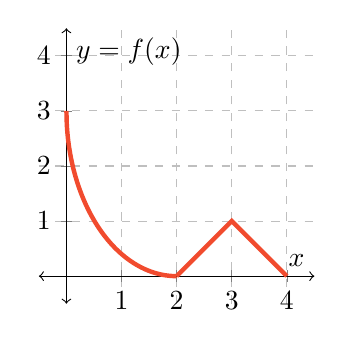
\begin{tikzpicture}[scale=1]
          \begin{axis}[
        %    axis y line = left,
        %    axis x line = bottom,
            xlabel={$x$},
	    ylabel={$y=f(x)$},
            xtick       = {1,2,3,4},
            xticklabels = {$1$,$2$,$3$,$4$},
            ytick       = {1,2,3,4},
            yticklabels = {$1$,$2$,$3$,$4$},
            samples     = 320,
            domain      = -1:5,
            restrict y to domain=-1:5,
            xmin = -0.5, xmax = 4.5,
            ymin = -0.5, ymax = 4.5,
            grid=both, grid style=dashed,
            width=2in, height=2in
          ]
          % pieces 1 and 2
          \addplot[domain=0:2, RedOrange, ultra thick, mark=none] {-((9-9/4*(x-2)^2)^(1/2))+3};

          
          
          \draw[RedOrange, ultra thick] (2,0) -- (3,1) -- (4,0);
          %\draw[RedOrange, ultra thick] (0,1) -- (1,1) -- (2,0) -- (3,3) -- (4,4);
          % piece 3

          % label
        \end{axis}
    \end{tikzpicture}
%    %
%    \hfill
%    %
}{
    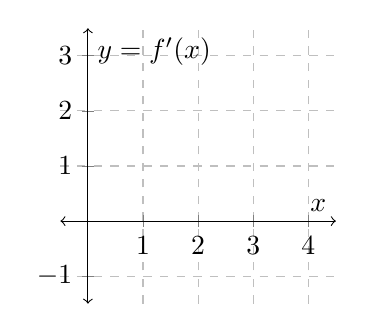
\begin{tikzpicture}[scale=1]
          \begin{axis}[
        %    axis y line = left,
        %    axis x line = bottom,
            xlabel={$x$},
                        ylabel={$y=f^{\prime}(x)$},
            xtick       = {1,2,3,4},
            xticklabels = {$1$,$2$,$3$,$4$},
            ytick       = {-1,1,2,3},
            yticklabels = {$-1$,$1$,$2$,$3$},
            samples     = 320,
            domain      = -1:5,
            restrict y to domain=-1:5,
            xmin = -0.5, xmax = 4.5,
            ymin = -1.5, ymax = 3.5,
            grid=both, grid style=dashed,
            width=2in, height=2in
          ]
        \end{axis}
    \end{tikzpicture}
%\end{minipage}\\
}

    \item Use the graph of $f$ and the table you built in part (a) to sketch the graph of $f'$ in the empty grid above for $0\leq x \leq 4$.
\end{enumerate}

\end{enumerate}
\vfill
\begin{enumerate}
\item[4.]\reversemarginpar\marginnote{\fbox{\bf\color{ForestGreen}D1}} Given to the right is a graph depicting within a container the relationship between the height $H$ (in cm) of water inside and the volume $L$ (in liter) of water filled into it.

\begin{enumerate}

\item[(a)] What does $\dfrac{H(40)-H(20)}{40-20}$ represent in this context? Sketch a line whose slope would represent this quantity geometrically in the grid to the right.

\end{enumerate}


%
\hfill
%
\begin{minipage}[t]{0.2\textwidth}
\begin{center}
        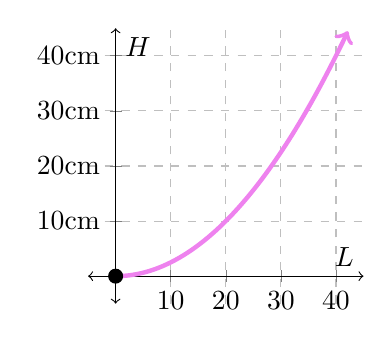
\begin{tikzpicture}[scale=1]
            \begin{axis}[
                %    axis y line = left,
                %    axis x line = bottom,
                    xlabel={$L$},
                    xtick       = {100,200,300,400},
                    xticklabels = {10,20,30,40},
                    ylabel={$H$},
                    ytick       = {1000,2000,3000,4000},
                    yticklabels = {10cm,20cm,30cm,40cm},
                    samples     = 160,
                    domain      = -50:450,
                    restrict y to domain=0:4500,
                    xmin = -50, xmax = 450,
                    ymin = -500, ymax = 4500,
                    grid=both, grid style=dashed,
                    width=2in, height=2in
                  ]
                  %\addplot[Violet, ultra thick, smooth] coordinates{ (0,0) (100,70) (200,1000) (300,1250) (400,4000) };
                  
                 \addplot[Violet, ultra thick, domain=0:450,->] {(x-0)^2/40};

                 \filldraw (0,0) circle (2.5pt);
            \end{axis}
        \end{tikzpicture}
\end{center}
\end{minipage}

\begin{enumerate}

\item[(b)] What are the units of measurement of the quantity $\dfrac{H(40)-H(20)}{40-20}$? $\dotfill$ 

\item[(c)] What does $\displaystyle\lim_{L\to20}\dfrac{H(L)-H(20)}{L-20}$ represent in this context? Sketch a line whose slope would represent this quantity geometrically in the grid above.

\vfill

\item[(d)] What are the units of measurement of the quantity $\displaystyle\lim_{L\to20}\dfrac{H(L)-H(20)}{L-20}$? $\dotfill$  

\end{enumerate}
\end{enumerate}

\end{document}